\chapter[Pr�cticas JPA]{Pr�cticas de modelado JPA}

\section{Enunciado}

Queremos modelar la base de datos de un conjunto de empresas que realizan proyectos para diversos clientes. Cada empresa se 
divide en departamentos que forman una jerarqu�a en �rbol anid�ndose los departmentos. Cada empleado trabaja en un departamento y 
cada departamento tiene un empleado que es responsable del mismo. 

Cada proyecto est� asignado a un departamento o a ninguno si no ha sido asignado a�n. En cada proyecto trabajan los empleados del 
departamento al que est� asignado el proyecto. Cada proyecto tiene asociado un cliente de la cartera global de clientes. 

Un proyecto tiene tres estados:
\begin{itemize}
\item En estudio
\item En desarrollo
\item Entregado
\item Finalizado 
\item Cancelado
\end{itemize} 

El estado inicial del proyecto es \emph{En estudio}. Cuando el proyecto se asocia a un departamento pasa al estado \emph{Desarrollo}.
El proyecto pasa el estado \emph{Entregado} cuando se entrega al cliente. Se debe registrar la fecha de entrega al cliente al alcanzar 
dicho estado. Cuando el cliente acepta el proyecto (despu�s de probarlo) el proyecto pasa al estado \emph{Finalizado}.
El cliente puede rechazar una entrega del proyecto con lo que el proyecto pasa al estado \emph{En desarrollo}.
Una vez que el proyecto est� entregado el cliente puede pedir mejoras para la siguiente versi�n del proyecto. En este caso el proyecto pasa
al estado \emph{En estudio} con un n� de versi�n superior y vuelven a realizar todas las fases.
En cualquier momento del proceso se puede cancelar un proyecto pasando el estado del mismo a \emph{Cancelado} y grab�ndose el motivo y la fecha 
de cancelaci�n.


\begin{figure}[h]
\centering
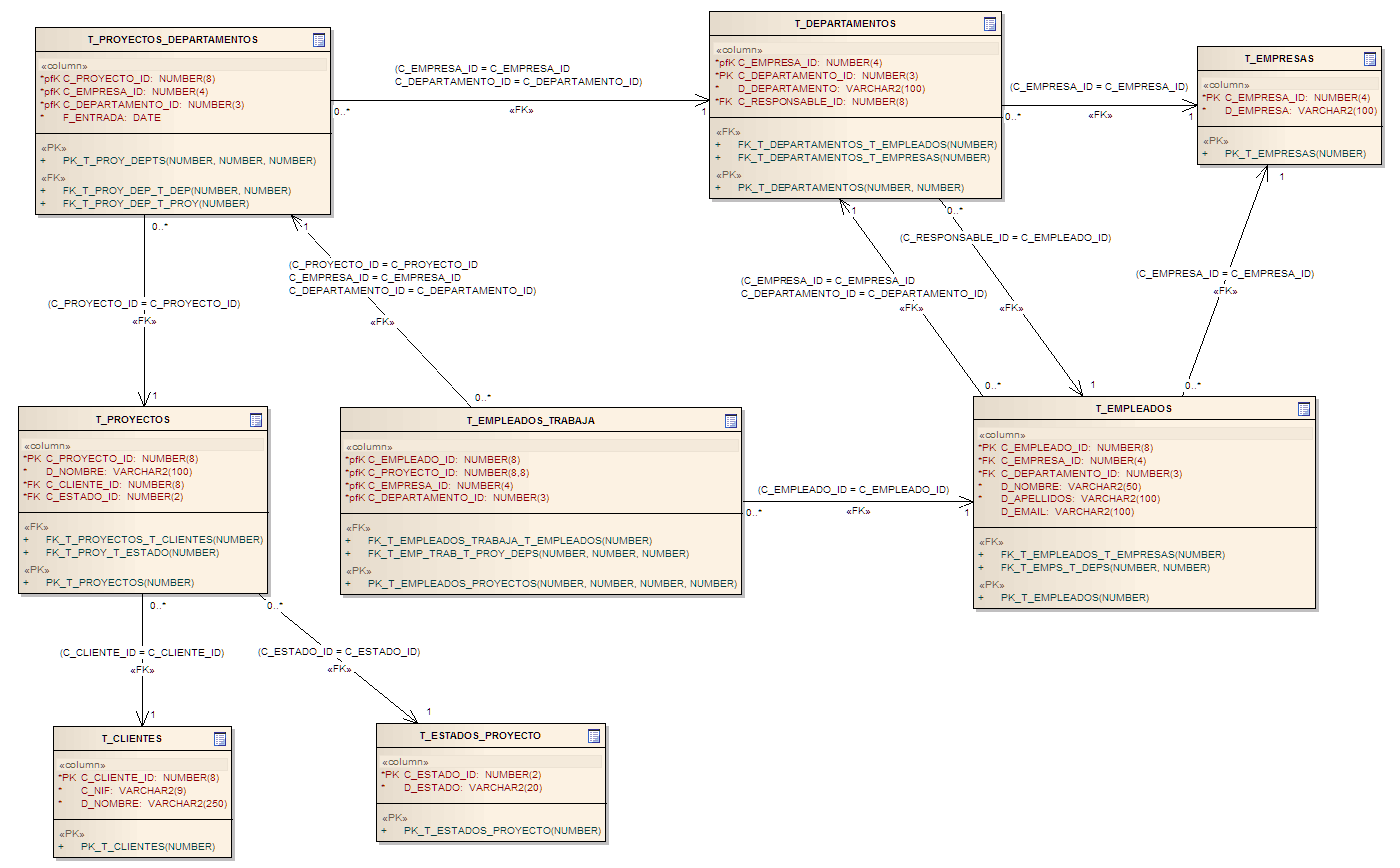
\includegraphics[width=6in]{cap03/PRUE.png}  
\caption{Modelo de datos de la pr�ctica}
\label{cap03:fig01}
\end{figure}
 
\section{Pr�ctica 1}
En esta pr�ctica vamos a modelar cada una de las entidades que aparecen en el enunciado:

\lstinputlisting[label=cliente.java,caption=Cliente.java]{../practicas/practica1/src/practica1/modelo/Cliente.java}
\lstinputlisting[label=departamento.java,caption=Departamento.java]{../practicas/practica1/src/practica1/modelo/Departamento.java}
\lstinputlisting[label=departamentoPK.java,caption=DepartamentoPK.java]{../practicas/practica1/src/practica1/modelo/DepartamentoPK.java}
\lstinputlisting[label=empleado.java,caption=Empleado.java]{../practicas/practica1/src/practica1/modelo/Empleado.java}
\lstinputlisting[label=empresa.java,caption=Empresa.java]{../practicas/practica1/src/practica1/modelo/Empresa.java}
\lstinputlisting[label=estado.java,caption=Estado.java]{../practicas/practica1/src/practica1/modelo/Empresa.java}
\lstinputlisting[label=proyecto.java,caption=Proyecto.java]{../practicas/practica1/src/practica1/modelo/Proyecto.java}
\lstinputlisting[label=proyectoDepartamentoPK.java,caption=ProyectoDepartamentoPK.java]{../practicas/practica1/src/practica1/modelo/ProyectoDepartamentoPK.java}
\lstinputlisting[label=proyectoDepartamento.java,caption=ProyectoDepartamento.java]{../practicas/practica1/src/practica1/modelo/ProyectoDepartamento.java}

\section{Pr�ctica 2}
